% Options for packages loaded elsewhere
\PassOptionsToPackage{unicode}{hyperref}
\PassOptionsToPackage{hyphens}{url}
\PassOptionsToPackage{dvipsnames,svgnames*,x11names*}{xcolor}
%
\documentclass[
  16pt,
]{article}
\usepackage{lmodern}
\usepackage{setspace}
\usepackage{amssymb,amsmath}
\usepackage{ifxetex,ifluatex}
\ifnum 0\ifxetex 1\fi\ifluatex 1\fi=0 % if pdftex
  \usepackage[T1]{fontenc}
  \usepackage[utf8]{inputenc}
  \usepackage{textcomp} % provide euro and other symbols
\else % if luatex or xetex
  \usepackage{unicode-math}
  \defaultfontfeatures{Scale=MatchLowercase}
  \defaultfontfeatures[\rmfamily]{Ligatures=TeX,Scale=1}
\fi
% Use upquote if available, for straight quotes in verbatim environments
\IfFileExists{upquote.sty}{\usepackage{upquote}}{}
\IfFileExists{microtype.sty}{% use microtype if available
  \usepackage[]{microtype}
  \UseMicrotypeSet[protrusion]{basicmath} % disable protrusion for tt fonts
}{}
\makeatletter
\@ifundefined{KOMAClassName}{% if non-KOMA class
  \IfFileExists{parskip.sty}{%
    \usepackage{parskip}
  }{% else
    \setlength{\parindent}{0pt}
    \setlength{\parskip}{6pt plus 2pt minus 1pt}}
}{% if KOMA class
  \KOMAoptions{parskip=half}}
\makeatother
\usepackage{xcolor}
\IfFileExists{xurl.sty}{\usepackage{xurl}}{} % add URL line breaks if available
\IfFileExists{bookmark.sty}{\usepackage{bookmark}}{\usepackage{hyperref}}
\hypersetup{
  pdftitle={An R package for synthesizing spatiotemporal point patterns for social and life science research - A user guide},
  colorlinks=true,
  linkcolor=Maroon,
  filecolor=Maroon,
  citecolor=Blue,
  urlcolor=blue,
  pdfcreator={LaTeX via pandoc}}
\urlstyle{same} % disable monospaced font for URLs
\usepackage[margin=1in]{geometry}
\usepackage{color}
\usepackage{fancyvrb}
\newcommand{\VerbBar}{|}
\newcommand{\VERB}{\Verb[commandchars=\\\{\}]}
\DefineVerbatimEnvironment{Highlighting}{Verbatim}{commandchars=\\\{\}}
% Add ',fontsize=\small' for more characters per line
\usepackage{framed}
\definecolor{shadecolor}{RGB}{248,248,248}
\newenvironment{Shaded}{\begin{snugshade}}{\end{snugshade}}
\newcommand{\AlertTok}[1]{\textcolor[rgb]{0.94,0.16,0.16}{#1}}
\newcommand{\AnnotationTok}[1]{\textcolor[rgb]{0.56,0.35,0.01}{\textbf{\textit{#1}}}}
\newcommand{\AttributeTok}[1]{\textcolor[rgb]{0.77,0.63,0.00}{#1}}
\newcommand{\BaseNTok}[1]{\textcolor[rgb]{0.00,0.00,0.81}{#1}}
\newcommand{\BuiltInTok}[1]{#1}
\newcommand{\CharTok}[1]{\textcolor[rgb]{0.31,0.60,0.02}{#1}}
\newcommand{\CommentTok}[1]{\textcolor[rgb]{0.56,0.35,0.01}{\textit{#1}}}
\newcommand{\CommentVarTok}[1]{\textcolor[rgb]{0.56,0.35,0.01}{\textbf{\textit{#1}}}}
\newcommand{\ConstantTok}[1]{\textcolor[rgb]{0.00,0.00,0.00}{#1}}
\newcommand{\ControlFlowTok}[1]{\textcolor[rgb]{0.13,0.29,0.53}{\textbf{#1}}}
\newcommand{\DataTypeTok}[1]{\textcolor[rgb]{0.13,0.29,0.53}{#1}}
\newcommand{\DecValTok}[1]{\textcolor[rgb]{0.00,0.00,0.81}{#1}}
\newcommand{\DocumentationTok}[1]{\textcolor[rgb]{0.56,0.35,0.01}{\textbf{\textit{#1}}}}
\newcommand{\ErrorTok}[1]{\textcolor[rgb]{0.64,0.00,0.00}{\textbf{#1}}}
\newcommand{\ExtensionTok}[1]{#1}
\newcommand{\FloatTok}[1]{\textcolor[rgb]{0.00,0.00,0.81}{#1}}
\newcommand{\FunctionTok}[1]{\textcolor[rgb]{0.00,0.00,0.00}{#1}}
\newcommand{\ImportTok}[1]{#1}
\newcommand{\InformationTok}[1]{\textcolor[rgb]{0.56,0.35,0.01}{\textbf{\textit{#1}}}}
\newcommand{\KeywordTok}[1]{\textcolor[rgb]{0.13,0.29,0.53}{\textbf{#1}}}
\newcommand{\NormalTok}[1]{#1}
\newcommand{\OperatorTok}[1]{\textcolor[rgb]{0.81,0.36,0.00}{\textbf{#1}}}
\newcommand{\OtherTok}[1]{\textcolor[rgb]{0.56,0.35,0.01}{#1}}
\newcommand{\PreprocessorTok}[1]{\textcolor[rgb]{0.56,0.35,0.01}{\textit{#1}}}
\newcommand{\RegionMarkerTok}[1]{#1}
\newcommand{\SpecialCharTok}[1]{\textcolor[rgb]{0.00,0.00,0.00}{#1}}
\newcommand{\SpecialStringTok}[1]{\textcolor[rgb]{0.31,0.60,0.02}{#1}}
\newcommand{\StringTok}[1]{\textcolor[rgb]{0.31,0.60,0.02}{#1}}
\newcommand{\VariableTok}[1]{\textcolor[rgb]{0.00,0.00,0.00}{#1}}
\newcommand{\VerbatimStringTok}[1]{\textcolor[rgb]{0.31,0.60,0.02}{#1}}
\newcommand{\WarningTok}[1]{\textcolor[rgb]{0.56,0.35,0.01}{\textbf{\textit{#1}}}}
\usepackage{graphicx}
\makeatletter
\def\maxwidth{\ifdim\Gin@nat@width>\linewidth\linewidth\else\Gin@nat@width\fi}
\def\maxheight{\ifdim\Gin@nat@height>\textheight\textheight\else\Gin@nat@height\fi}
\makeatother
% Scale images if necessary, so that they will not overflow the page
% margins by default, and it is still possible to overwrite the defaults
% using explicit options in \includegraphics[width, height, ...]{}
\setkeys{Gin}{width=\maxwidth,height=\maxheight,keepaspectratio}
% Set default figure placement to htbp
\makeatletter
\def\fps@figure{htbp}
\makeatother
\setlength{\emergencystretch}{3em} % prevent overfull lines
\providecommand{\tightlist}{%
  \setlength{\itemsep}{0pt}\setlength{\parskip}{0pt}}
\setcounter{secnumdepth}{-\maxdimen} % remove section numbering

\title{An R package for synthesizing spatiotemporal point patterns for
social and life science research - A user guide}
\author{Monsuru Adepeju\footnote{Big Data Centre, Manchester
  Metropolitan University, Manchester, M156BH, UK,
  \href{mailto:m.adepeju@mmu.ac.uk}{\nolinkurl{m.adepeju@mmu.ac.uk}}}}
\date{\texttt{Date:}~\\
\texttt{2022-03-20}}

\begin{document}
\maketitle
\begin{abstract}
With increasingly limited availability of fine-grained spatially and
temporally stamped point data, the \texttt{stppSim} provides an
alternative source of data for a wide range of research in social and
life sciences. It generates artificial spatio-temporal (ST) point
patterns through the integration of microsimulation and agent-based
models. Allows a user to define the behaviours of a set of `walkers'
(agents, objects, persons, etc,) whose interactions with the spatial
(landscape) and the temporal domains produce new point events. Based on
the resulting point cloud, the ST patterns can be measured and utilized
for spatial and/or temporal model testings and evaluations.
\end{abstract}

{
\hypersetup{linkcolor=}
\setcounter{tocdepth}{3}
\tableofcontents
}
\setstretch{1.5}
\hypertarget{introduction}{%
\subsection{Introduction}\label{introduction}}

In many research context, access to fine-grained spatiotemporal (ST)
point data have been severely restricted due to privacy concerns. The
\texttt{R-stppSim} package has been designed to address this challenge
by presenting a framework that is capable of mimicking a real-life data
through the integration of microsimulation and agent-based techniques.
The framework comprises a set of `walkers' (agents, objects, persons,
etc.) with modifiable movement and interaction properties, constructed
within specified spatial and temporal domains. As the framework produces
new point events, in accordance with a user setting, a defined ST
pattern emerges at both the local and global levels.

The package contains two main functions for synthesizing new datasets;
(i) \texttt{psim\_artif} and (ii) \texttt{psim\_real}. The
\texttt{psim\_artif} synthesizes ST point patterns from scratch. That
is, the simulation is entirely based on a user's setting. On the other
hand, \texttt{psim\_real} synthesizes ST point patterns based on a
sample (or a sparse version) of a real data. The function first learns
(or extracts) the certain ST characteristics of the sample data, and
extrapolates to produce full dataset. The potential application fields
for \texttt{stppSim} include criminology, epidemiology, and wildlife
science.

\hypertarget{simulation-parameters}{%
\subsection{Simulation Parameters}\label{simulation-parameters}}

The simulation parameters are in relation to three elements, namely; the
`\texttt{walkers\ (agents)}', the \texttt{landscape} (spatial), and the
\texttt{temporal\ dimension}. The parameters are described as follow:

\hypertarget{walkers-agents.}{%
\subsubsection{Walkers (agents).}\label{walkers-agents.}}

The walkers are defined primarily by the following characteristics:

\begin{itemize}
\tightlist
\item
  \textbf{\emph{Origins}} - The walkers emanate from a set of origins
  that are distributed randomly across the landscape or origins defined
  from a sample of real point data. Origins are defined in terms of
  \texttt{xy} coordinates. In criminological application, a human
  offender can be modelled as a walker originating from his residence
  (origin). The \texttt{origins} of walkers typically exhibit two types
  of concentration: \texttt{nucleated} and \texttt{dispersed}
  (\texttt{ref}). A \texttt{nucleated} concentration is the one in which
  all origins concentrate around one focal point, while a
  \texttt{dispersed} concentration has no one particular focus, but
  could have multiple mini focal points (see fig.~1).
\end{itemize}

\begin{figure}

\hfill{}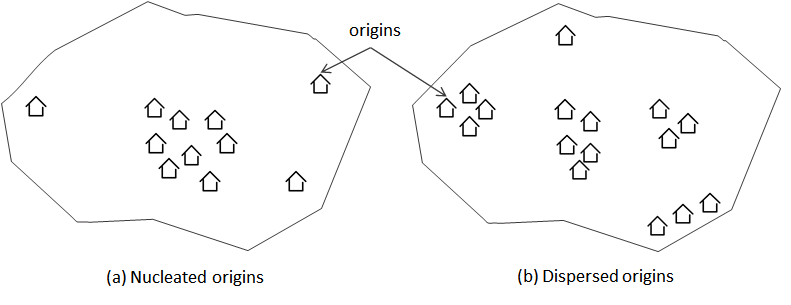
\includegraphics[width=0.9\linewidth,height=1\textheight]{C:/Users/monsu/Documents/GitHub/stppSim backup/figs/origins} 

\caption{Interactive predictive hotspot map}\label{fig:fig1}
\end{figure}

\begin{itemize}
\item
  \textbf{\emph{Movement}} - Walkers are configured to move in any
  direction and to be aware of obstacles (restrictions) on their path.
  The movements are controlled primarily by an in-built transition
  matrix (TM) definig two transitional states, namely; an
  \texttt{exploratory} state (in which a walker is merely exploring the
  environment) and a \texttt{performative} state (in which a walker is
  performing an action). The stochastic properties of the TM ensure
  variations in the behavioral patterns amongst the walkers. In order to
  switch from one state to the next, a categorical distribution is
  assigned to the latent state variable \(z_{it}\). So, every time step
  may be assigned to a movement behaviour state, independent of the
  previous state: \[z_t \sim Categorical(\Psi{_{1t}}, \Psi{_{2t}})\]
  Such that \(\Psi{_{i}}\) = Pr\((z_t = i)\), where \(\Psi{_{i}}\) is
  the fixed probability of being in state \(i\) at time \(t\), and
  \(\sum_{i=1}^{z}\Psi{_{i}}=1\)
\item
  \textbf{\emph{Spatial threshold, k}} - The perception range of a
  walker at a given location. The parameter \texttt{k} is generally
  updated as a walker moves to a new location. A natural method for
  choosing the smoothing parameter is to plot out the data choose the
  estimate that is most in accordance with one's prior ideas about the
  \texttt{k} value. For many applications this approach will be
  perfectly satisfactory. To simulate data from sample data sets, the
  optimal value of \texttt{k} can also be extracted using a
  \href{https://www.taylorfrancis.com/books/mono/10.1201/9781315140919/density-estimation-statistics-data-analysis-silverman}{plug-in
  function}.
\item
  \textbf{\emph{Steps}} - The maximum step taken by a walker as he moves
  from one location to another. This defines the speed of a walker
  across the space. The \texttt{steps} should be carefully defined,
  especially, when movements are restricted along narrow paths, such as
  route network (a step argument must be smaller than the width of the
  paths.
\item
  \textbf{\emph{Proportional ratios}} - Defines the percentage of total
  events emanating from a small number of origins (i.e., most active
  origins). A \texttt{20:80} proportional ratios implies that 20\% of
  origins (walkers) generates 80\% of the point events.
\end{itemize}

\hypertarget{landscape-spatial}{%
\subsubsection{Landscape (spatial)}\label{landscape-spatial}}

The followings are the key properties of a landscape:

\begin{itemize}
\tightlist
\item
  \textbf{\emph{Boundary}} - A landscape is bounded - defined by a
  polygon shapefile (\texttt{poly}) or by the spatial extent of the
  sample point data.
\item
  \textbf{\emph{Restrictions}} - Defined as a raster layer. Typically
  defines two features: (i) Areas outside the boundary with the maximum
  restriction level (i.e., \texttt{1} - implying no movement), and (ii)
  Features within the boundary serving as obstructions to movement,
  e.g., certain land use type or topography, such as a fenced place and
  hills.
\item
  \textbf{\emph{Focal points}} - Locations around which there are higher
  concentration of opportunities (to event occurrences). Relatively
  higher activities in/around these locations, such as the centres of
  any city.
\end{itemize}

\hypertarget{temporal-dimension}{%
\subsubsection{Temporal dimension}\label{temporal-dimension}}

The following parameters define the temporal dimension:

\begin{itemize}
\tightlist
\item
  \textbf{\emph{Long-term trend}} - Defines the long-term direction of
  the time series to be simulated. This can be \texttt{stable},
  \texttt{rising} or \texttt{falling}. If either \texttt{rising} or
  \texttt{falling}, the slope can be \texttt{gentle} or \texttt{steep}.
  Only specified when simulating from scratch.
\item
  \textbf{\emph{Short-term patterns}} - Defines the short-term variation
  in events total over time. This is controlled by specifying the first
  seasonal peak point of the time series. A \texttt{90} day first peak
  implies a seasonal cycle of \texttt{180} days. Also, specified when
  simulating from scratch.
\item
  \textbf{\emph{time bin}} - Time to reset all walkers.
\end{itemize}

\hypertarget{installation-of-stppsim}{%
\subsection{\texorpdfstring{Installation of
\texttt{stppSim}}{Installation of stppSim}}\label{installation-of-stppsim}}

From an R console, type:

\begin{Shaded}
\begin{Highlighting}[]
\KeywordTok{install.packages}\NormalTok{(}\StringTok{"stppSim"}\NormalTok{)}
\CommentTok{\#To install the developmental version of the package, type:}
\NormalTok{remotes}\OperatorTok{::}\KeywordTok{install\_github}\NormalTok{(}\StringTok{"MAnalytics/stppSim"}\NormalTok{)}
\end{Highlighting}
\end{Shaded}

Note: \texttt{remotes} is an extra package that needed to be installed
prior to the running of this code.

\begin{Shaded}
\begin{Highlighting}[]
\CommentTok{\#Now, load the package,}
\KeywordTok{library}\NormalTok{(stppSim)}
\end{Highlighting}
\end{Shaded}

\hypertarget{synthesizing-stpp-from-scratch}{%
\subsection{\texorpdfstring{Synthesizing \texttt{stpp} from
scratch}{Synthesizing stpp from scratch}}\label{synthesizing-stpp-from-scratch}}

To simulate point patterns from scratch, the argument \texttt{n\_events}
specifies the number of points to simulate. It is recommended to input a
vector of values, instead of a single value. For example,
\texttt{n\_events\ =\ c(200,\ 500,\ 1000,\ 2000)}. This saves the user
the time from having to synthesize new data. \textbf{\emph{Note}}: the
specification of \texttt{n\_events} input has little or no impacts on
the computational time (See the manual for further details).

\hypertarget{example-using-a-restricted-landscape}{%
\subsubsection{Example using a restricted
landscape}\label{example-using-a-restricted-landscape}}

Given a boundary shapefile \{e.g., data(\texttt{camden\_boundary}\} and
land use features with restriction values \{e.g., data(\texttt{landuse})
- \texttt{Leisure} (0.5); \texttt{Sports} (0.7); and \texttt{Green}
(0.9)\}, the ST point pattern can be generated as follows:

\begin{Shaded}
\begin{Highlighting}[]
\CommentTok{\#Using datasets that come with the package;}
\KeywordTok{data}\NormalTok{(camden\_boundary)}
\KeywordTok{data}\NormalTok{(landuse)}

\CommentTok{\#specifyings say 3 data sizes}
\NormalTok{pt\_sizes =}\StringTok{ }\KeywordTok{c}\NormalTok{(}\DecValTok{200}\NormalTok{, }\DecValTok{1000}\NormalTok{, }\DecValTok{2000}\NormalTok{)}

\NormalTok{artif\_stpp <{-}}\StringTok{ }\KeywordTok{psim\_artif}\NormalTok{(}\DataTypeTok{n\_events=}\NormalTok{pt\_sizes, }\DataTypeTok{start\_date =} \StringTok{"2021{-}01{-}01"}\NormalTok{,}
  \DataTypeTok{poly=}\NormalTok{camden\_boundary, }\DataTypeTok{n\_origin=}\DecValTok{50}\NormalTok{, }\DataTypeTok{resistance\_feat =}\NormalTok{ landuse,}
  \DataTypeTok{field =} \StringTok{"rValue1"}\NormalTok{,}
  \DataTypeTok{n\_foci=}\DecValTok{5}\NormalTok{, }\DataTypeTok{foci\_separation =} \DecValTok{10}\NormalTok{, }\DataTypeTok{conc\_type =} \StringTok{"dispersed"}\NormalTok{,}
  \DataTypeTok{p\_ratio =} \DecValTok{20}\NormalTok{, }\DataTypeTok{s\_threshold =} \DecValTok{50}\NormalTok{, }\DataTypeTok{step\_length =} \DecValTok{20}\NormalTok{,}
  \DataTypeTok{trend =} \StringTok{"stable"}\NormalTok{, }\DataTypeTok{first\_pDate=}\OtherTok{NULL}\NormalTok{,}
  \DataTypeTok{slope =} \OtherTok{NULL}\NormalTok{,}\DataTypeTok{show.plot=}\OtherTok{FALSE}\NormalTok{, }\DataTypeTok{show.data=}\OtherTok{FALSE}\NormalTok{)}
\end{Highlighting}
\end{Shaded}

To preview the output:

\begin{Shaded}
\begin{Highlighting}[]
\KeywordTok{head}\NormalTok{(artif\_stpp)}
\end{Highlighting}
\end{Shaded}

Users should explore the impacts of different arguments, including the
\texttt{n\_origin}, \texttt{foci\_separation}, \texttt{trend}
\{\texttt{stable},\texttt{increasing} or \texttt{decreasing}\}, and
\texttt{conc\_type} \{\texttt{nucleated} or \texttt{dispersed}\}.

Exploring the results using visualization:

\begin{itemize}
\tightlist
\item
  \textbf{Figure 1abc - spatial patterns of 200, 1000. 2000 data points}
\end{itemize}

The corresponding temporal pattern of the data can be visualized as
follows:

\begin{itemize}
\tightlist
\item
  \textbf{Figure 2 - temporal patterns of 200, 1000. 2000 data points}
\end{itemize}

\hypertarget{synthesizing-stpp-from-a-sample-real-dataset}{%
\subsection{\texorpdfstring{Synthesizing \texttt{stpp} from a sample
real
dataset}{Synthesizing stpp from a sample real dataset}}\label{synthesizing-stpp-from-a-sample-real-dataset}}

Here, we are going to extract 30\% random sample the \texttt{Theft}
crime of Camden, then utilize the sample to synthesize a \texttt{full}
data size.

\begin{Shaded}
\begin{Highlighting}[]
\KeywordTok{data}\NormalTok{(camden\_crimes)}

\CommentTok{\#get the \textquotesingle{}theft\textquotesingle{} crime}
\NormalTok{theft <{-}}\StringTok{ }\NormalTok{camden\_crimes }\OperatorTok{\%>\%}
\StringTok{  }\KeywordTok{filter}\NormalTok{(type }\OperatorTok{==}\StringTok{ "Theft"}\NormalTok{)}

\CommentTok{\#specify the proportion to extract}
\NormalTok{sample\_size <{-}}\StringTok{ }\FloatTok{0.3} \CommentTok{\#i.e. 30\% of real data}

\KeywordTok{set.seed}\NormalTok{(}\DecValTok{1000}\NormalTok{)}
\NormalTok{dat\_sample <{-}}\StringTok{ }\NormalTok{theft[}\KeywordTok{sample}\NormalTok{(}\DecValTok{1}\OperatorTok{:}\KeywordTok{nrow}\NormalTok{(theft),}
  \KeywordTok{round}\NormalTok{((sample\_size }\OperatorTok{*}\StringTok{ }\KeywordTok{nrow}\NormalTok{(theft)), }\DataTypeTok{digits=}\DecValTok{0}\NormalTok{),}
  \DataTypeTok{replace=}\OtherTok{FALSE}\NormalTok{),}\DecValTok{1}\OperatorTok{:}\DecValTok{3}\NormalTok{]}

\CommentTok{\#As a user would not normally know the actual size of }
\CommentTok{\#the real full data, therefore, we would assume \textasciigrave{}n\_events\textasciigrave{}}
\CommentTok{\#to be \textasciigrave{}2000\textasciigrave{}. In practice, a user should infer }
\CommentTok{\#the input size from any available (similar) data }
\CommentTok{\#from the study area.}

\CommentTok{\#Now, simulate}
\NormalTok{sim\_fullData <{-}}\StringTok{ }\KeywordTok{psim\_real}\NormalTok{(}\DataTypeTok{n\_events=}\DecValTok{2000}\NormalTok{, }\DataTypeTok{ppt=}\NormalTok{dat\_sample,}
  \DataTypeTok{start\_date =} \OtherTok{NULL}\NormalTok{, }\DataTypeTok{poly =} \OtherTok{NULL}\NormalTok{, }\DataTypeTok{s\_threshold =} \OtherTok{NULL}\NormalTok{,}
  \DataTypeTok{step\_length =} \DecValTok{20}\NormalTok{, }\DataTypeTok{n\_origin=}\DecValTok{50}\NormalTok{, resistance\_feat, }\DataTypeTok{field=}\OtherTok{NA}\NormalTok{,}
  \DataTypeTok{p\_ratio=}\DecValTok{20}\NormalTok{, }\DataTypeTok{crsys =} \StringTok{"EPSG:27700"}\NormalTok{)}

\CommentTok{\#plot(dat\_sample$x, dat\_sample$y) \#preview}
\end{Highlighting}
\end{Shaded}

Preview the resulting data using visualization approach (above).

\hypertarget{comparing-simulated-data-and-full-real-data} real data size.
The visual approach involves the comparison of \texttt{heat\ maps}
derived from the aggregation of the datasets to a square grid system
(250m x 250m). The statistical approach involves computing the
\texttt{pearson\ coefficient} to compares the two datasets.

\begin{itemize}
\tightlist
\item
  Visual approach
\end{itemize}

** Spatial Figure 1a (heat map of simulated data) Figure 1b (heat map of
full real data)

** Temporal Figure 2a (Time series plot of simulated data) Figure 2b
(Time series plot of full real data)

\begin{itemize}
\tightlist
\item
  Statistical approach
\end{itemize}

Flattening the 2D square grids (above) and then apply Pearson
correlation:

\begin{Shaded}
\begin{Highlighting}[]
\CommentTok{\#corr}

\KeywordTok{cor}\NormalTok{(sim, real)}
\end{Highlighting}
\end{Shaded}

\hypertarget{discussion}{%
\subsection{Discussion}\label{discussion}}

This vignette has demonstrated the basic utility of \texttt{stppSim}
package for generating fine-grained spatiotemporal point patterns, (1)
from scratch and (2) from a sample of real data sets. The parameters of
the three simulation elements: the `Walkers (agents)', the landscape
(spatial), and the time dimension should be modified in accordance with
the research questions at hand. The package has a wide potential areas
of applications. Examples of objects with similar objectives as walkers
(as defined in this package) include, human offenders, foraging animals
and disease carriers, in victimization, Wildlife, and epidemiological
studies, respectively. We will continue to update the package for wider
application.

We encourage users to report any bugs encountered while using the
package so that they can be fixed immediately. Welcome contributions to
this package which will be acknowledged accordingly.

\end{document}
